\section{Bewertung}
\label{sec:Bewertung}
Im folgenden sind Komponente aufgelistet, welche im Kontext des Kapitels \ref{sec:Stand der Technik} erarbeitet wurden und einen Variantenentscheid mit sich bringen. Dazu werden messbare Kriterien definiert, gewichtet und die einzelnen Varianten daran gemessen.

Den Varianten wird eine Punktzahl auf einer linearen Skala von 1 bis 5 zugewiesen.

\subsection{Routing über offene Flächen}
\label{eval:Routing über offene Flächen}

Das Kapitel \ref{solution:Routing über offene Flächen} hat zwei Algorithmen hervorgebracht, namentlich \nameref{solution:Visibility Graph} und \nameref{solution:Spider-Web Graph}, welche im Folgenden analysiert werden.

\subsubsection{Kriterien}
\label{sub:Kriterien}

\paragraph{Verarbeitungszeit}\label{criteria:Verarbeitungszeit}~\\
Der aktuelle Import der \ac{OSM}-Daten der Schweiz ins System Tourpl \cite{hsr_tourpl}, ein Produkt des Geometa Lab der HSR \cite{geometa_lab_hsr}, dauert 2 Stunden. Diese Zeitdauer soll nicht überschritten werden. Die Verarbeitungszeit wird bewertet auf einer Skala von 1 (2 Stunden) bis 5 (0 Minuten).


\paragraph{zusätzliche Datenmenge}\label{criteria:zusätzliche Datenmenge}~\\
Die Algorithmen generieren zusätzliche Geometrien. Da die öffentlichen Plätze nur einen kleinen Teil der Kartendaten bilden, soll die zusätzliche Datenmenge keinen signifikaten Teil ausmachen. Die zusätzliche Datenmenge im Verhältnis zur originalen Datei wird bewertet auf einer Skala von 1 (1\%) bis 5 (0\%).


\paragraph{Natürlichkeit}\label{criteria:Natürlichkeit}~\\
% TODO Verweis auf Definition in Graser-Paper
Für die Natürlichkeit einer Route ist es schwer, messbare Kriterien zu definieren. Als eine natürliche Route versteht man, wenn man auf direktem Weg über den Platz geht und keine Umwege macht. Treten Hindernisse auf dem Platz auf, widerspricht es einem natürlichen Fussgänger-Verhalten, wenn man direkt aufs Hindernis zu läuft und dieses am Rande umgeht. Um trotzdem ein Fazit ziehen zu können, werden 3 Plätze (Helvetiaplatz in Zürich, Fischmarktplatz in Rapperswil-Jona und der Bahnhofplatz in Bern) untersucht. Dabei wird für beide Varianten eine interaktive Routing-Oberfläche an Probanden zu Verfügung gestellt. Die Probanden haben die Möglichkeit, selbst Routen über den Platz zu setzen. In Abbildung \ref{fig:algorithm-example-routes} sind einige Routen beispielhaft dargestellt. Danach bewerten die Probanden die vorhin definierte Natürlichkeit mit Punkten von 1 bis 5. Als massgeblicher Vergleichswert wird der Durchschnitt der Bewertungen aller Probanden genommen.

\begin{figure}[ht]
    \centering
    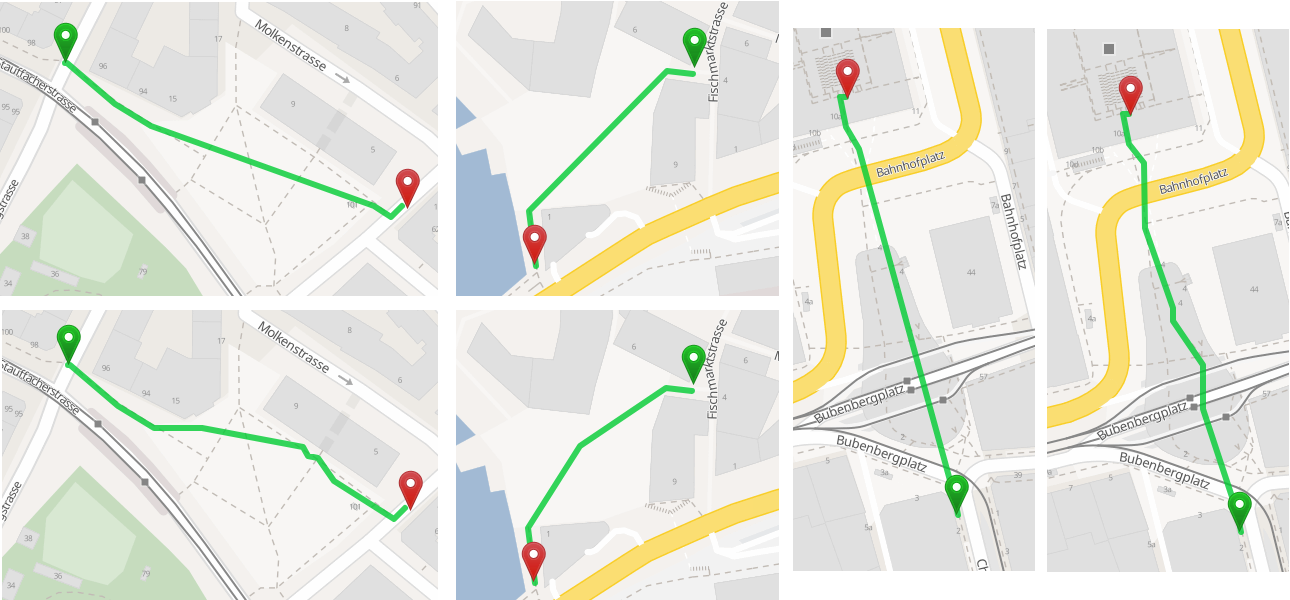
\includegraphics[width=1\linewidth]{technicalreport/img/algorithm-comparison-routes}
    \caption[Beispielhafte Routen für Natürlichkeits-Test]{Beispielhafte Routen über die drei getesteten Flächen; Jeweils oben bzw. links Visibility Graph, unten bzw. rechts Spiderweb Graph}
    \label{fig:algorithm-example-routes}
\end{figure}


\subsubsection{Resultate}
\label{sub:Resultate}

Die Vorverarbeitung wurde auf einem Rechner mit einem Intel i7 2600k Prozessor und Fedora 26 als Betriebssystem ausgeführt.

Für die Vergleichswerte der Verarbeitungszeit und der zusätzlichen Datenmenge wird die Datei \emph{switzerland-exact.osm} \cite{osm_data_switzerland}, Stand 12.11.17, verwendet. Im \ac{OSM}-Format ist die Datei 6.3 GB gross.


\begin{figure}[ht]
    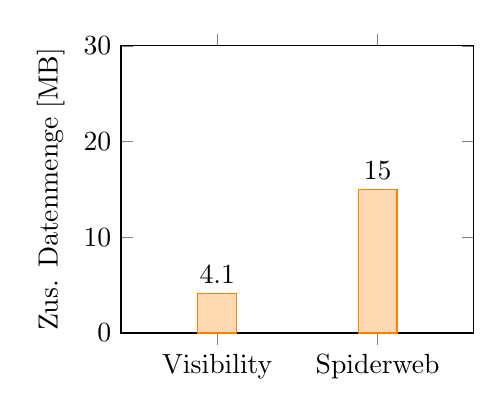
\begin{tikzpicture}
        \begin{axis}[
            ybar,
            width=0.5\textwidth,
            bar width=14pt,
            ylabel={Zus. Datenmenge [MB]},
            ymin=0,
            ymax=30,
            symbolic x coords={Visibility,Spiderweb},
            xtick=data,
            enlarge x limits=0.6, % pull bars together
            nodes near coords,
            nodes near coords align={vertical},
            every node near coord/.append style={color=black}
        ] 
            \addplot[style={orange,fill=orange!30!white}]
                coordinates {(Visibility,4.1) (Spiderweb,15)};
        \end{axis}
    \end{tikzpicture}%
    ~%
    % ~ to not break the line 
    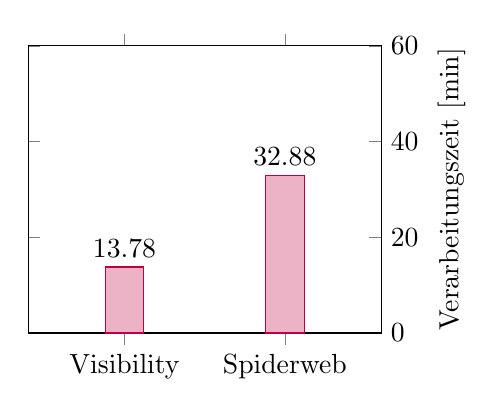
\begin{tikzpicture}
        \begin{axis}[
            ybar,
            width=0.5\textwidth,
            bar width=14pt,
            ylabel={Verarbeitungszeit [min]},
            ylabel near ticks, 
            yticklabel pos=right, % axis label on the right
            ymin=0,
            ymax=60,
            symbolic x coords={Visibility,Spiderweb},
            xtick=data,
            enlarge x limits=0.6, % pull bars together
            nodes near coords,
            nodes near coords align={vertical},
            every node near coord/.append style={color=black},
        ] 
            \addplot[style={purple,fill=purple!30!white}]
                coordinates {(Visibility,13.78) (Spiderweb,32.88)};
        \end{axis}
    \end{tikzpicture}

    \caption[Diagramm Datenmenge / Verarbeitungszeit]{Vergleich der zusätzlichen Datenmenge und der Verarbeitungszeit von Visibility Graph und Spiderweb Graph}
    \label{chart:datenmenge_laufzeit_vergleich}
\end{figure}
    

\paragraph{Verarbeitungszeit}\label{result:Verarbeitungszeit}~\\
Die Vorverarbeitung wurde mit beiden Algorithmen auf der Test-Datei ausgeführt und dabei die benötigte Zeit gemessen. Die Zeit für den ersten Schritt, das Importieren der \ac{OSM}-Daten, wird dabei abgezogen, da dies unabhängig vom jeweiligen Algorithmus ist. Die Resultate sind in Tabelle \ref{Resultat: Verarbeitungszeit} dargestellt.

\begin{table}[H]
    \centering
    \caption{Resultat: Verarbeitungszeit (ohne Initialer Import der Daten)}
    \label{Resultat: Verarbeitungszeit}
    \begin{tabular}{lll}
        & \textbf{Visiblity Graph} & \textbf{Spiderweb Graph}     \\
        Verarbeitungszeit  &        13m47s                   & 32m53s    \\
        %  5 - ((t / 2h)*4)
        \textbf{Bewertung 1-5} &    4.54                     &  3.90
    \end{tabular}
\end{table}


\paragraph{zusätzliche Datenmenge}\label{result:zusätzliche Datenmenge}~\\
Tabelle \ref{table: zusätzliche Datenmenge} zeigt die zusätzliche Datenmenge im \ac{OSM}-Format, die durch die Vorverarbeitung mit dem jeweiligen Algorithmus entstanden ist, verglichen mit der Dateigrösse der \ac{OSM}-Datei vor der Vorverarbeitung.

\begin{table}[H]
    \centering
    \caption{Resultat: zusätzliche Datenmenge}
    \label{table: zusätzliche Datenmenge}
    \begin{tabular}{lll}
        & \textbf{Visibility Graph} & \textbf{Spiderweb Graph} \\
        \textbf{zusätzliche Datenmenge} & 4.13 MB                    & 15.1 MB  \\  
        in Prozent der Originalgrösse   & 0.06\%                     & 0.24\%   \\
        \textbf{Bewertung 1-5}          & 4.76                       & 4.04
    \end{tabular}
\end{table}

\paragraph{Natürlichkeit}\label{result:Natürlichkeit}~\\
Für die Evaluation wurde die Bewertung der Natürlichkeit mit fünf Probanden durchgeführt. Die einzelnen Bewertungen sind in Tabelle \ref{table:Resultat Natürlichkeit} abgebildet. In Abbildung \ref{chart:natürlichkeit_vergleich} sind die durchschnittlichen Bewertungen pro Platz und Algorithmus dargestellt.

\begin{figure}[ht]
    \centering
    \begin{tikzpicture}
        \begin{axis}[
            ybar,
            width=0.8\textwidth,
            bar width=14pt,
            ylabel={Durchschnittliche Bewertung},
            ymin=1,
            ymax=5,
            symbolic x coords={Helvetiaplatz,Fischmarktplatz,Bahnhofplatz Bern},
            xtick=data,
            enlarge x limits=0.2, % pull bars together
            nodes near coords,
            nodes near coords align={vertical},
            every node near coord/.append style={color=black}
        ]            
            \addplot[style={blue, fill=blue!30!white},postaction={pattern=north east lines}] coordinates 
                {(Helvetiaplatz,3.6) (Fischmarktplatz,3.2) (Bahnhofplatz Bern,3.2)};
            \addplot [style={red, fill=red!30!white},postaction={pattern=dots}] coordinates 
                {(Helvetiaplatz,3.6) (Fischmarktplatz,3.4) (Bahnhofplatz Bern,3.2)};
            \legend{Visibility Graph,Spiderweb Graph}
        \end{axis}
    \end{tikzpicture}%

    \caption[Diagramm Natürlichkeit von Visibility / Spiderweb Graph]{Durchschnittliche Bewertungen der Natürlichkeit auf den verschiedenen Plätzen}
    \label{chart:natürlichkeit_vergleich}
\end{figure}


\begin{table}[ht]
    \centering
    \caption{Resultat: Natürlichkeit}
    \label{table:Resultat Natürlichkeit}
    \begin{tabular}{lll}
        & \textbf{Visibility Graph} & \textbf{Spiderweb Graph} \\
        \textbf{Helvetiaplatz}   &                          &                          \\
        Proband 1                & 4                        & 3                        \\
        Proband 2                & 3                        & 4                        \\
        Proband 3                & 4                        & 3                        \\
        Proband 4                & 4                        & 4                        \\
        Proband 5                & 3                        & 4                        \\
        \textbf{Fischmarktplatz} &                          &                          \\
        Proband 1                & 4                        & 3                        \\
        Proband 2                & 4                        & 3                        \\
        Proband 3                & 3                        & 4                        \\
        Proband 4                & 2                        & 3                        \\
        Proband 5                & 3                        & 4                        \\
        \textbf{Bahnhofplatz Bern} &                        &                          \\
        Proband 1                & 4                        & 3                        \\
        Proband 2                & 3                        & 4                        \\
        Proband 3                & 4                        & 2                        \\
        Proband 4                & 3                        & 4                        \\
        Proband 5                & 2                        & 3                        \\
        \textbf{Resultat}        & \textbf{3.33}               & \textbf{3.4}                       
    \end{tabular}
\end{table}

\subsubsection{Auswertung und Schlussfolgerung}
\label{result:Auswertung und Schlussfolgerung}

Die einzelnen Werte sind in Tabelle \ref{table:Resultat Evaluation Flächen-Algorithmus} zusammen gefasst und gewichtet. Es zeigt sich, dass der Visibility Graph knapp besser abschneidet, der Unterschied ist allerdings sehr gering und nicht eindeutig.

Bei der Bewertung der Natürlichkeit durch Probanden ergaben sich einige Erkenntnisse. So bewerteten einige Probanden eine direkte Route mit etwas ``scharfen'' Ecken - wie sie der Visibility Graph erzeugt - natürlicher, während andere die etwas kurvigeren Routen des Spiderweb Graphs bevorzugten.

Abschliessend kann man sagen, dass beide Algorithmen gute Resultate bringen. Wenn die Verarbeitungszeit wichtig ist, bringt der Visibility Graph Vorteile, der Spiderweb Graph erzeugt dafür tendenziell die etwas natürlicheren Routen.

\begin{table}[ht]
    \centering
    \caption{Resultat der Evaluation Flächen-Algorithmus}
    \label{table:Resultat Evaluation Flächen-Algorithmus}
    \begin{tabular}{lllll}
            \hline
            \textbf{ID} & \textbf{Titel}         & \textbf{\begin{tabular}[c]{@{}l@{}}Relatives Gewicht \\ (0-1)\end{tabular}} & \textbf{Visibility Graph} & \textbf{Spiderweb Graph} \\ \hline
            1           & \nameref{criteria:Verarbeitungszeit}      & 0.3       & 4.54 / 1.36                   & 3.9 / 1.17                   \\
            2           & \nameref{criteria:zusätzliche Datenmenge} & 0.2       & 4.76 / 0.95                   & 4.04 / 0.81                  \\
            3           & \nameref{criteria:Natürlichkeit}          & 0.5       & 3.33 / 1.67                   & 3.4 / 1.7                    \\ \hline
            \multicolumn{3}{l}{\textbf{Total}}                                  & \textbf{12.6 / 3.98}         & \textbf{11.36 / 3.68}
     \end{tabular}               
\end{table}

